\documentclass[10pt,journal,twoside]{IEEEtran}

\usepackage{graphicx}
\usepackage{amsmath}
\usepackage{amsthm}
\usepackage{amssymb}
\usepackage{booktabs}
\usepackage{cite}
\usepackage{url}
\usepackage[hidelinks]{hyperref}

\newtheorem{theorem}{Theorem}[section]
\newtheorem{lemma}[theorem]{Lemma}
\newtheorem{corollary}[theorem]{Corollary}
\newtheorem{proposition}[theorem]{Proposition}
\newtheorem{definition}[theorem]{Definition}
\newtheorem{assumption}[theorem]{Assumption}
\theoremstyle{remark}
\newtheorem{remark}{Remark}[section]

\newcommand{\negl}{\mathsf{negl}}
\newcommand{\CS}{\mathit{CS}}

\title{Proof of Commitment: Consensus Through
	Sustained Participation}

\author{Homayoun~Maleki,~\IEEEmembership{}
	Nekane~Sainz,~\IEEEmembership{}
	Jon~Legarda,~\IEEEmembership{}
	and~Igor~Santos-Grueiro%
	\thanks{H. Maleki, N. Sainz, and J. Legarda are with
		DeustoTech, University of Deusto, Bilbao, Spain
		(e-mail: h.maleki@deusto.es).}%
	\thanks{I. Santos-Grueiro is with UNIR,
		Logro\~{n}o, Spain.}%
	\thanks{Manuscript submitted to IEEE Transactions on
		Dependable and Secure Computing.}%
	\thanks{Simulation code available at:
		\url{https://github.com/homayoun1220/pocmt-simulation}.}}

\begin{document}
	\maketitle
	\IEEEpeerreviewmaketitle
	
	%%=============================================================
	\begin{abstract}
		Permissionless consensus has traditionally derived influence
		from accumulated resources, most notably computational power
		in Proof of Work and financial stake in Proof of Stake.
		While effective for Sybil resistance, these approaches tie
		consensus influence to resource accumulation, creating
		persistent incentives for concentration.
		
		This paper explores an alternative foundation in which
		influence emerges from sustained participation over time.
		We present \emph{Proof of Commitment} (PoCmt), a
		permissionless consensus mechanism where validators
		gradually build a commitment score through recurring
		protocol engagement across consecutive time windows.
		Block-production opportunities are allocated according to
		this accumulated commitment, allowing influence to develop
		progressively through continued participation rather than
		through the acquisition of external resources.
		
		PoCmt introduces a participation-based model in which
		influence is earned independently by each identity over
		time, making long-term participation the primary source of
		consensus power. Building on this model, we construct a
		commitment-weighted leader election mechanism and prove
		backbone-style safety, liveness, and commitment-proportional
		fairness under partial synchrony. Security derives from
		structural participation constraints embedded in the
		participation model itself.
		
		Seven simulation experiments demonstrate behavior consistent
		with the theoretical analysis across churn, offline, and
		adversarial environments. The results show that influence
		formation is governed by sustained participation capacity
		rather than by identity replication, while commitment
		dynamics converge to the rates predicted by the model.
		
		These results establish sustained participation as a
		structurally distinct and formally grounded basis for
		permissionless consensus—one that decouples influence from
		resource accumulation and offers a concrete alternative path
		toward long-term decentralization.
	\end{abstract}
	
	\begin{IEEEkeywords}
		permissionless consensus, sustained participation,
		commitment score, Sybil resistance, backbone security,
		decentralization
	\end{IEEEkeywords}
	
	
	%%=============================================================
	\section{Introduction}
	\label{sec:intro}
	
	Decentralization is the foundational promise of blockchain.
	No single entity should dominate; influence should be
	distributed, and power should not concentrate.
	Yet the two paradigms that have come to define permissionless
	consensus---Proof of Work
	(PoW)~\cite{nakamoto2008bitcoin,garay2015bitcoin,
		garay2020analysis} and Proof of Stake
	(PoS)~\cite{kiayias2017ouroboros,david2018praos,
		badertscher2018genesis}---have produced, in practice,
	the opposite.
	Mining pools controlling the majority of global hash
	power~\cite{gencer2018decentralization}, and liquid staking
	protocols accumulating a third of all staked
	ETH~\cite{wahrstatter2023lido}: these are not accidents of
	implementation.
	They are the predictable outcome of building consensus on
	\emph{parallelizable resources}---hardware and capital
	that can be freely pooled and redistributed across
	arbitrarily many identities without proportional recurring
	cost.
	Our companion paper~\cite{maleki2025scarcity} examines
	this structural property of parallelizable resources and
	shows that protocols built on such a foundation cannot
	enforce linear Sybil cost, regardless of how their rules
	are designed.
	PoCmt addresses this by replacing the resource class
	itself---from one that can be parallelized to one that
	cannot.
	
	\subsection{Commitment as a Resource}
	
	This paper asks a different question: what if influence
	required not \emph{owning} something, but
	\emph{continuously doing} something?
	
	The intuition is simple.
	A validator that participates in the protocol today---
	responding to challenges, engaging with the network---
	and does so again tomorrow, and the day after, and for
	months thereafter, is doing something that cannot be
	replicated in bulk.
	Each act of participation must be performed per identity,
	per time window.
	It cannot be stockpiled in advance, outsourced to a single
	process without limit, or transferred from one identity to
	another.
	What makes this resource scarce is not its quantity
	but its structure: each identity must earn it
	separately, in each window, and there is no shortcut---
	no bulk purchase, no delegation, no way to compress
	weeks of participation into a single transaction.
	
	An entity wishing to sustain influence across $s$
	identities under such a model must supply $s$ independent
	acts of engagement per window---not once, but repeatedly,
	for as long as influence is desired.
	The cost scales linearly with identity count and
	participation horizon, not with the depth of a balance
	sheet.
	This is the structural inversion that breaks the
	concentration dynamic: capital can be pooled;
	commitment cannot.
	
	We present \emph{Proof of Commitment} (PoCmt), a
	permissionless consensus mechanism that instantiates this
	idea formally.
	Validators accumulate a \emph{Commitment Score} through
	recurring protocol engagement across consecutive time
	windows.
	Block-production rights are allocated proportionally to
	this score.
	Influence grows gradually through sustained participation
	and cannot be acquired instantaneously through capital
	injection or hardware scaling.
	
	\subsection{This Work}
	
	We develop PoCmt from first principles: a formal model
	of participation as a non-aggregable resource, a complete
	consensus protocol built on that foundation, and a security
	analysis proving backbone-style safety, liveness, and
	commitment-proportional fairness under partial
	synchrony~\cite{dwork1988partialsync}.
	Security follows from structural participation constraints
	and an honest channel majority; it does not depend on
	the scarcity of any aggregable resource class.
	Seven analytical experiments confirm that the model
	behaves as the analysis predicts.
	
	\subsection{Contributions}
	
	\begin{enumerate}
		
		\item \textbf{Participation-Based Influence Model
			(Section~\ref{sec:resource}).}
		A formal model in which consensus influence derives from
		sustained per-identity participation.
		We identify the structural properties that make
		participation non-aggregable and show that the cost of
		sustaining $s$ identities over $T$ windows grows as
		$\Omega(sT)$, independently of capital or hardware.
		
		\item \textbf{Commitment Score Framework
			(Section~\ref{sec:score}).}
		A three-component Commitment Score combining
		participation history~($H_v$), protocol
		compliance~($P_v$), and availability~($U_v$).
		We prove that honest aggregate weight exhibits positive
		drift over adversarial weight under an honest channel
		majority (Lemma~\ref{lem:drift}), with exponential
		concentration guarantees
		(Corollary~\ref{cor:stabilization}).
		
		\item \textbf{PoCmt Protocol
			(Section~\ref{sec:protocol}).}
		A complete permissionless consensus protocol with
		VRF-based commitment-weighted leader election,
		block proposal and validation, multiplicative slashing,
		and two finality modes.
		
		\item \textbf{Backbone-Style Security Analysis
			(Section~\ref{sec:security}).}
		Formal proofs of the common-prefix property
		(Theorem~\ref{thm:safety}), liveness
		(Theorem~\ref{thm:liveness}), and
		commitment-proportional fairness
		(Lemma~\ref{lem:fairness}) under partial synchrony.
		Full derivations appear in
		Appendices~\ref{app:drift}--\ref{app:safety}.
		
		\item \textbf{Analytical Validation
			(Section~\ref{sec:eval}).}
		Seven simulation experiments testing phase transition
		in adversarial leader share, non-amplification under
		identity replication, sensitivity to the servicing
		bound~$\tau$ and honest surplus~$\varepsilon$,
		robustness under churn, offline recovery, and direct
		measurement of commitment drift.
		
	\end{enumerate}
	
	\subsection{Organization}
	
	Section~\ref{sec:related} surveys related work.
	Section~\ref{sec:model} establishes the system model.
	Section~\ref{sec:resource} develops the participation
	resource model.
	Section~\ref{sec:score} defines the Commitment Score.
	Section~\ref{sec:protocol} presents the protocol.
	Section~\ref{sec:security} proves the security results.
	Section~\ref{sec:eval} reports simulation experiments.
	Section~\ref{sec:discussion} discusses scope and limitations.
	Section~\ref{sec:conclusion} concludes.
	%%=============================================================
	\section{Related Work}
	\label{sec:related}
	
	%%---------------------------------------------------------------
	\subsection{Accumulated-Resource Consensus}
	\label{ssec:rw-accumulated}
	
	Douceur~\cite{douceur2002sybil} established that
	permissionless systems cannot resist Sybil attacks without
	binding influence to a costly resource.
	The dominant instantiations tie that resource to
	accumulated holdings.
	
	\emph{Proof of Work.}
	Nakamoto~\cite{nakamoto2008bitcoin} tied block-production
	probability to computational effort; backbone-style
	security was established by Garay et
	al.~\cite{garay2015bitcoin,garay2020analysis} and extended
	to partial synchrony by Pass and Shi~\cite{pass2017hybrid}.
	Selfish-mining~\cite{eyal2018selfish} and
	stubborn-mining~\cite{nayak2020stubborn} analyses show how
	rational deviations concentrate influence in practice;
	Gencer et al.~\cite{gencer2018decentralization} empirically
	confirmed 53\% pool concentration in Bitcoin.
	
	\emph{Proof of Stake.}
	Kiayias et al.~\cite{kiayias2017ouroboros} gave the first
	provably secure PoS protocol.
	Ouroboros Praos~\cite{david2018praos} extended this to
	adaptive corruption; Genesis~\cite{badertscher2018genesis}
	addressed dynamic availability; Badertscher et
	al.~\cite{badertscher2021stake} gave a UC-composable
	treatment.
	Algorand~\cite{gilad2017algorand} combines stake-weighted
	sortition with BFT agreement for low-latency finality.
	Wahrstätter et al.~\cite{wahrstatter2023lido} document
	liquid staking driving a single protocol to over 32\% of
	staked ETH.
	
	\emph{Economic and structural limits.}
	Bonneau et al.~\cite{bonneau2015sok} survey Bitcoin-style
	incentive and concentration issues.
	Budish et al.~\cite{budish2024economic} formalize the
	economic limits of capital-based security.
	Lewis-Pye and Roughgarden~\cite{lewispye2023permissionless}
	characterize which consensus properties are achievable
	under different resource and participation models.
	Our companion paper~\cite{maleki2025scarcity} establishes
	the structural result underlying PoCmt: any consensus
	protocol whose weighting resource can be freely aggregated
	admits sublinear Sybil cost, regardless of protocol rules.
	PoCmt responds by replacing the resource class rather than
	adjusting the protocol.
	
	%%---------------------------------------------------------------
	\subsection{Sequential Work and Time-Based Resources}
	\label{ssec:rw-sequential}
	
	Proofs of Sequential Work~\cite{cohen2018sequential,
		mahmoody2013sequential} and Verifiable Delay
	Functions~\cite{boneh2018vdf,wesolowski2019vdf} enforce
	wall-clock lower bounds on individual computations and
	support delay-based randomness beacons~\cite{syta2017drand}.
	These are useful building blocks but do not resolve the
	aggregation problem: an adversary sustaining $s$ identities
	simply provisions $s$ independent machines and evaluates
	$s$ delay functions in parallel.
	The dominant cost remains capital expenditure on hardware,
	not elapsed time.
	PoCmt's participation model addresses this gap directly by
	capping the number of identities a single process can
	service per window, independently of hardware investment.
	
	%%---------------------------------------------------------------
	\subsection{Alternative Resource Models}
	\label{ssec:rw-alt}
	
	Proof-of-Space~\cite{dziembowski2015spacemint} derives
	influence from disk capacity;
	Proof-of-Elapsed-Time~\cite{abadi2016poet,chen2017poetanalysis}
	relies on trusted execution environments;
	Proof-of-Useful-Work~\cite{ball2017proofs} ties influence
	to externally valuable computation.
	These approaches reduce energy consumption or hardware
	barriers relative to PoW, but their underlying resources
	remain divisible and transferable, and therefore remain
	subject to the aggregation dynamics documented
	in~\cite{maleki2025scarcity}.
	
	Graph-based Sybil defenses---SybilGuard~\cite{yu2006sybilguard}
	and SybilInfer~\cite{danezis2009sybilinfer}---constrain
	Sybil identity placement via social network structure.
	They address where adversarial identities appear, not the
	recurring cost of sustaining them, and are complementary
	to PoCmt rather than competitive.
	
	%%---------------------------------------------------------------
	\subsection{Participation and Identity-Binding Mechanisms}
	\label{ssec:rw-participation}
	
	Proof-of-Personhood proposals~\cite{borges2017popp,
		ford2020pseudonym} and deployed
	systems---Worldcoin~\cite{worldcoin2023},
	BrightID~\cite{brightid2022}, Gitcoin
	Passport~\cite{gitcoin2023},
	PoPCoin~\cite{ford2019popcoin}---increase the cost of
	\emph{creating} an identity through biometric or social
	ceremony.
	Human-work proposals~\cite{blocki2016humanwork,kopp2016umine}
	replace computational puzzles with cognitive tasks.
	CAPTCHA~\cite{vonahn2003captcha} gates account creation
	by exploiting perception gaps between humans and solvers.
	
	PoCmt differs from all of these in two respects.
	First, it enforces a \emph{recurring} per-window cost
	rather than a one-time admission cost: an adversary that
	has established $s$ identities must continue supplying
	$s$ independent participation acts per window to retain
	influence.
	Second, PoCmt makes no assumption about human superiority
	over automated solvers; security derives from structural
	properties of the participation resource, not from any
	human-versus-machine capability gap.
	Table~\ref{tab:related} positions PoCmt relative to the
	prior landscape.
	
	%%---------------------------------------------------------------
	\subsection{Formal Consensus Security}
	\label{ssec:rw-formal}
	
	PoCmt adopts the partial synchrony model of Dwork, Lynch,
	and Stockmeyer~\cite{dwork1988partialsync} and the
	backbone proof methodology of Garay et
	al.~\cite{garay2015bitcoin,garay2020analysis}.
	Pass and Shi~\cite{pass2017sleepy} introduced the sleepy
	model capturing dynamic validator availability, directly
	relevant to PoCmt's churn analysis.
	Ren~\cite{ren2019analysis} provided tighter
	confirmation-depth bounds for Nakamoto-style protocols.
	PBFT~\cite{castro1999pbft} and
	HotStuff~\cite{yin2019hotstuff,abraham2020hotstuff} inform
	the optional BFT finality gadget.
	The proof novelty in PoCmt lies not in the backbone
	methodology but in the arguments connecting participation
	dynamics (Lemma~\ref{lem:drift}) to classical chain
	properties (Theorem~\ref{thm:safety}).
	
	\begin{table}[t]
		\centering
		\caption{Positioning of PoCmt relative to prior work.
			\emph{Persistent} = recurring per-window cost.
			\emph{Non-aggregable} = influence cannot be pooled
			across identities.
			\emph{Solver-agnostic} = no human-superiority
			assumption.}
		\label{tab:related}
		\renewcommand{\arraystretch}{1.15}
		\resizebox{\columnwidth}{!}{%
			\begin{tabular}{@{}lccc@{}}
				\toprule
				\textbf{Mechanism}
				& \textbf{Persistent}
				& \textbf{Non-aggregable}
				& \textbf{Solver-agnostic} \\
				\midrule
				PoW~\cite{nakamoto2008bitcoin}
				& \checkmark & $\times$ & \checkmark \\
				PoS~\cite{kiayias2017ouroboros}
				& \checkmark & $\times$ & \checkmark \\
				VDF~\cite{boneh2018vdf}
				& \checkmark & $\times$ & \checkmark \\
				PoP~\cite{borges2017popp}
				& $\times$ & $\times$ & $\times$ \\
				PoPCoin~\cite{ford2019popcoin}
				& \checkmark & $\times$ & $\times$ \\
				Human-Work~\cite{blocki2016humanwork}
				& $\times$ & Partial & $\times$ \\
				CAPTCHA~\cite{vonahn2003captcha}
				& $\times$ & $\times$ & $\times$ \\
				\midrule
				\textbf{PoCmt (this work)}
				& \checkmark & \checkmark & \checkmark \\
				\bottomrule
		\end{tabular}}
	\end{table}
	%%=============================================================
	\section{System Model}
	\label{sec:model}
	
	Table~\ref{tab:notation} summarises the core notation.
	
	%%---------------------------------------------------------------
	\subsection{Execution Model}
	\label{ssec:exec}
	
	Protocol execution is \emph{round-based}.
	Time proceeds in discrete \emph{rounds} $r = 1, 2, \ldots$
	of fixed wall-clock duration $\delta > 0$.
	Each active validator receives all messages delivered in
	round $r$, performs local computation, and sends at most
	one message to each other validator.
	
	\begin{definition}[Epoch and Participation Window]
		\label{def:timescales}
		A \emph{consensus epoch} $t$ consists of $R_e \in
		\mathbb{N}_{>0}$ consecutive rounds.
		A \emph{participation window} $d$ consists of
		$E \in \mathbb{N}_{>0}$ consecutive epochs
		($R_w = E \cdot R_e$ rounds).
		We write $\mathrm{ep}(r)$ and $\mathrm{win}(r)$ for
		the epoch and window containing round $r$, and
		$d(t) = \lceil t / E \rceil$.
	\end{definition}
	
	The two-timescale structure is necessary: consensus messages
	are exchanged at epoch granularity while participation
	challenges are scored at window granularity, keeping
	participation-based influence constant within a window and
	preventing rapid amplification through short bursts.
	Window boundaries are globally computable from the protocol
	transcript without trusted clock infrastructure.
	
	%%---------------------------------------------------------------
	\subsection{Network Model}
	\label{ssec:network}
	
	We adopt the \emph{partial synchrony} model of
	Dwork, Lynch, and Stockmeyer~\cite{dwork1988partialsync}.
	
	\begin{definition}[Partial Synchrony --- DLS Model]
		\label{def:partialsync}
		There exists an unknown \emph{Global Stabilization Time}
		$\mathrm{GST} \geq 0$ such that:
		\begin{enumerate}
			\item[\textbf{(N1)}] For $r < \mathrm{GST}$, the
			adversary may delay, reorder, or suppress messages,
			subject to eventual delivery by round
			$\mathrm{GST} + \Delta_e$.
			\item[\textbf{(N2)}] For $r \geq \mathrm{GST}$,
			every honest message sent in round $r$ is received
			by all honest validators by round $r + \Delta_e$.
		\end{enumerate}
		$\mathrm{GST}$ is unknown; $\Delta_e$ is a public parameter.
	\end{definition}
	
	\begin{remark}
		\label{rem:gst}
		Safety holds for all $r \geq 0$.
		Liveness holds for $r \geq \mathrm{GST} + \Delta_e$.
		The adversary may know $\mathrm{GST}$; our proofs
		do not rely on the contrary.
	\end{remark}
	
	%%---------------------------------------------------------------
	\subsection{Participants and Identities}
	\label{ssec:identity}
	
	The validator set is \emph{open and dynamic}.
	Any entity joins by generating a fresh key pair
	$(pk_v, sk_v)$ under an existentially unforgeable
	signature scheme~\cite{goldreich2001foundations};
	no admission cost or trusted authority is required.
	
	\begin{definition}[Validator Sets]
		\label{def:valsets}
		For round $r$, let $\mathcal{V}(r) = \mathcal{H}(r)
		\cup \mathcal{A}(r)$ where $\mathcal{H}(r)$ is the set
		of honest validators and $\mathcal{A}(r)$ the corrupted
		set; the two are disjoint.
	\end{definition}
	
	We place no a priori bound on $|\mathcal{V}(r)|$ or
	$|\mathcal{A}(r)|$; security guarantees are stated in terms
	of \emph{participation capacity} rather than identity count.
	
	%%---------------------------------------------------------------
	\subsection{Adversarial Model}
	\label{ssec:adversary}
	
	\paragraph{Corruption model.}
	The adversary selects $\mathcal{C} \subseteq \mathcal{V}(1)$
	before execution begins (static corruption), following the
	standard backbone
	assumption~\cite{garay2015bitcoin,pass2017hybrid}.
	Within each round, the adversary is \emph{rushing}: it
	observes all honest messages before deciding corrupted
	validators' messages.
	All parties are PPT algorithms parametrised by $\lambda$;
	security guarantees hold except with probability
	$\negl(\lambda)$.
	
	\begin{remark}[Adaptive corruption]
		\label{rem:adaptive}
		Adaptive corruption requires the UC framework and
		significantly increases proof complexity; we defer
		this to future work (Section~\ref{sec:discussion}).
	\end{remark}
	
	\paragraph{Participation capacity constraints.}
	Regardless of computational or financial resources,
	the adversary cannot:
	\begin{enumerate}
		\item[\textbf{(C1)}] credit a valid proof for
		identity $v$ to any $v' \neq v$;
		\item[\textbf{(C2)}] carry a proof from window $d$
		to any $d' > d$;
		\item[\textbf{(C3)}] service more than $\tau \in O(1)$
		identities per window per independent process.
	\end{enumerate}
	These constraints are enforced structurally by the
	participation resource model (Section~\ref{sec:resource}),
	independently of adversarial computational power.
	
	%%---------------------------------------------------------------
	\subsection{Honest Participation Assumption}
	\label{ssec:honest}
	
	Security is stated over \emph{participation channels}
	rather than commitment weight to avoid circularity:
	commitment weight is a protocol output; channels are a
	structural input constraint.
	
	\begin{assumption}[$\varepsilon$-Honest Channel Majority]
		\label{asm:majority}
		Let $n_{\mathcal{H}}(d)$ and $m_{\mathcal{A}}(d)$
		denote, respectively, the number of honest participation
		channels and adversarial participation processes in
		window $d$.
		There exist $\varepsilon > 0$ and
		$D_0 \in \mathbb{N}$ such that for all $d \geq D_0$:
		\[
		n_{\mathcal{H}}(d) \;\geq\; (1 + \varepsilon)\,
		m_{\mathcal{A}}(d).
		\]
	\end{assumption}
	
	\begin{remark}[Channel majority versus stake majority]
		\label{rem:majority_justified}
		This assumption is weaker than honest-majority
		assumptions in PoW/PoS in two respects.
		First, channels cannot be acquired instantaneously:
		reaching $m_{\mathcal{A}}$ adversarial channels requires
		operating them across at least $D_0$ windows, a cost
		that cannot be front-loaded.
		Second, the assumption is over processes, not identities:
		each process services at most $\tau$ identities~(C3),
		so unbounded identity creation does not help beyond
		the $\tau m_{\mathcal{A}}$ ceiling.
		Lemma~\ref{lem:drift} derives weight majority from
		these structural constraints rather than asserting it
		directly.
	\end{remark}
	
	%%---------------------------------------------------------------
	\subsection{Notation}
	\label{ssec:notation}
	
	\begin{table}[t]
		\caption{Core notation.}
		\label{tab:notation}
		\renewcommand{\arraystretch}{1.2}
		\begin{tabular}{@{}ll@{}}
			\toprule
			\textbf{Symbol} & \textbf{Meaning} \\
			\midrule
			$\lambda$              & Security parameter \\
			$r$                    & Protocol round \\
			$t$                    & Consensus epoch ($R_e$ rounds) \\
			$d$                    & Participation window ($E$ epochs) \\
			$d(t)$                 & Window containing epoch $t$ \\
			$\mathcal{V}(r)$       & Active validators at round $r$ \\
			$\mathcal{H}(r)$       & Honest validators at round $r$ \\
			$\mathcal{A}(r)$       & Corrupted validators at round $r$ \\
			$v$                    & Validator identity (public key) \\
			$\tau$                 & Servicing bound: max identities per
			process per window \\
			$m_{\mathcal{A}}(d)$   & Adversarial participation processes
			in window $d$ \\
			$n_{\mathcal{H}}(d)$   & Honest participation channels in
			window $d$ \\
			$H_v(d)$               & Participation commitment of $v$
			in window $d$ \\
			$P_v(t)$               & Protocol compliance of $v$ at
			epoch $t$ \\
			$U_v(t)$               & Availability of $v$ at epoch $t$ \\
			$\CS_v(t)$             & Commitment weight of $v$ at
			epoch $t$ \\
			$W_{\mathcal{H}}(t)$   & Total honest commitment weight \\
			$W_{\mathcal{A}}(t)$   & Total adversarial commitment weight \\
			$W_{\mathrm{tot}}(t)$  & $W_{\mathcal{H}}(t)+W_{\mathcal{A}}(t)$ \\
			$C(s,T)$               & Min.\ channel-windows to sustain
			$s$ identities over $T$ windows \\
			$\varepsilon$          & Honest channel surplus
			(Assumption~\ref{asm:majority}) \\
			$\mathrm{GST}$         & Global Stabilization Time \\
			$\Delta_e$             & Post-GST message delay bound (rounds) \\
			\bottomrule
		\end{tabular}
	\end{table}
	
	%%=============================================================
	\section{Participation-Based Influence Model}
	\label{sec:resource}
	
	This section develops the formal model underlying PoCmt's
	approach to consensus influence.
	We proceed in four steps: we define the structural
	properties that make a participation resource
	non-aggregable; we model the capacity constraints that
	follow from those properties; we state the resource
	assumptions that the deployed mechanism must satisfy;
	and we derive the cost bound connecting the resource
	model to the security analysis.
	
	%%---------------------------------------------------------------
	\subsection{Non-Aggregable Participation}
	\label{ssec:tpi}
	
	In PoW and PoS, a single entity can direct a fixed
	resource base across arbitrarily many identities without
	proportional additional cost.
	The key structural difference in PoCmt is that
	participation cannot be aggregated in this way.
	We formalize the conditions that make this so.
	
	\begin{definition}[Non-Aggregable Participation Resource]
		\label{def:tpi}
		A \emph{participation resource} $\mathcal{R}$ admits
		non-aggregable influence if there exists a publicly
		executable verification predicate
		$\mathsf{Ver} : \mathcal{ID} \times \mathbb{N} \times
		\{0,1\}^* \to \{0,1\}$
		satisfying the following three properties for all
		validators $v$, windows $d$, and security
		parameter $\lambda$:
		
		\begin{enumerate}
			\item[\textbf{(R1)}] \textbf{Identity binding.}
			$\mathsf{Ver}(v, d, \pi) = 1$ implies
			$\mathsf{Ver}(v', d, \pi) = 0$ for all $v' \neq v$,
			except with probability $\negl(\lambda)$.
			A valid participation proof cannot be credited to
			any identity other than the one that produced it.
			
			\item[\textbf{(R2)}] \textbf{Window locality.}
			$\mathsf{Ver}(v, d, \pi) = 1 \Rightarrow
			\mathsf{Ver}(v, d', \pi) = 0$ for all $d' \neq d$.
			Participation must be renewed each window;
			proofs cannot be carried forward or reused.
			
			\item[\textbf{(R3)}] \textbf{Bounded concurrent
				servicing.}
			There exists $\tau \in \mathbb{N}_{>0}$ such that
			any single process $p$ produces at most $\tau$
			valid proofs across distinct identities per window:
			\[
			\bigl|\{v : \mathsf{Ver}(v, d, \pi_p^v) = 1\}\bigr|
			\leq \tau,
			\]
			independently of $p$'s computational resources or
			the number of identities it attempts to service.
		\end{enumerate}
		
		Resources satisfying (R1)--(R3) are called
		\emph{time-per-identity (TPI) resources}.
	\end{definition}
	
	Properties (R1) and (R2) together prevent influence from
	being transferred between identities or banked across
	windows without fresh participation.
	Property (R3) is the aggregation barrier: a single process
	can supply participation for at most $\tau$ identities per
	window, so sustaining $s$ identities requires at least
	$\lceil s/\tau \rceil$ independent processes.
	Capital and hardware can increase the quality or speed of
	individual participation but cannot bypass this ceiling.
	
	\begin{remark}[Contrast with existing resource classes]
		\label{rem:tpi-vs-parallel}
		PoW and PoS fail (R2) and (R3): a fixed resource base
		is reusable across windows and can be subdivided to
		service arbitrarily many identities simultaneously.
		VDFs~\cite{boneh2018vdf} satisfy a sequential-time
		constraint within a single execution but fail (R3):
		an adversary provisions $s$ independent machines and
		runs $s$ delay functions in parallel at no additional
		per-identity recurring cost.
		This class of resource enforces (R3) at the process
		level, requiring proportionally more independent
		processes for each additional identity.
	\end{remark}
	
	\begin{remark}[Solver agnosticism]
		\label{rem:solver-agnostic}
		Properties (R1)--(R3) constrain the \emph{structure}
		of participation, not the identity of the solver.
		Whether proofs are generated by humans, automated
		agents, or hybrid systems is orthogonal to the cost
		analysis; only the process-level throughput ceiling
		$\tau$ matters for security.
	\end{remark}
	
	%%---------------------------------------------------------------
	\subsection{Participation Capacity Model}
	\label{ssec:capacity-model}
	
	We now model the concrete capacity constraints that
	follow from Definition~\ref{def:tpi} (the participation
	resource properties).
	
	A \emph{participation process} is an independent
	computational unit capable of generating valid
	participation proofs on behalf of one or more identities.
	The key quantities are:
	\begin{itemize}
		\item $\tau$: the \emph{servicing bound}---the maximum
		number of distinct identities a single process can
		validly service per window, enforced by (R3).
		\item $m$: the number of independent participation
		processes an entity operates.
		\item $s$: the number of identities the entity wishes
		to sustain with nontrivial commitment.
	\end{itemize}
	
	The relationship between these quantities determines
	whether influence can be aggregated.
	If a single process could service an unbounded number of
	identities ($\tau \to \infty$), one entity with one
	process could sustain arbitrarily many identities---the
	PoW/PoS regime.
	Property (R3) caps this: to sustain $s$ identities, an
	entity needs at least $\lceil s/\tau \rceil$ processes.
	When $\tau = O(1)$, this means $\Omega(s)$ processes
	are required, making the cost of sustaining many
	identities grow proportionally with $s$.
	
	This capacity model is the bridge between the abstract
	resource definition and the security analysis: it
	translates (R3) into a concrete bound on adversarial
	proof production, which in turn bounds adversarial
	commitment growth.
	
	%%---------------------------------------------------------------
	\subsection{Participation Resource Assumptions}
	\label{ssec:po}
	
	We assume that the participation resource deployed in
	PoCmt satisfies three structural properties.
	This is analogous to assuming a collision-resistant hash
	function in PoW: the assumption characterizes the
	required properties of the mechanism without prescribing
	a specific construction.
	Deployed participation systems have demonstrated the
	operational feasibility of recurring per-identity
	participation bounds at scale~\cite{pinetwork2019};
	a formal cryptographic construction is an open
	problem (Section~\ref{ssec:disc-open}).
	
	\begin{assumption}[Participation Resource]
		\label{asm:po}
		The deployed participation resource satisfies,
		for all validators $v$, windows $d$, and
		identities $v' \neq v$:
		\begin{enumerate}
			\item[\textbf{(A1)}] \textbf{Identity binding.}
			A valid proof for $v$ in window $d$ cannot be
			credited to any $v' \neq v$, except with
			probability $\negl(\lambda)$.
			Enforces (R1).
			
			\item[\textbf{(A2)}] \textbf{Window locality.}
			Proofs cannot be precomputed before challenge
			issuance and expire at the window boundary.
			Enforces (R2).
			
			\item[\textbf{(A3)}] \textbf{Bounded concurrent
				servicing.}
			There exists $\tau > 0$ such that any single
			process produces valid proofs for at most $\tau$
			distinct identities per window, independently of
			computational power.
			Enforces (R3).
		\end{enumerate}
	\end{assumption}
	
	\begin{remark}[Conditionality]
		\label{rem:po-assumption}
		Assumption~\ref{asm:po} plays the same role as the
		honest-majority assumption in PoS or the
		collision-resistance assumption in PoW: a structural
		precondition on the deployment environment, not a
		consequence of protocol rules.
		All security results in Section~\ref{sec:security}
		are conditional on Assumption~\ref{asm:po}.
	\end{remark}
	
	Concrete mechanisms satisfying Assumption~\ref{asm:po}
	include per-session serialization (one active challenge
	per session token), device-bound attestation (a hardware
	enclave enforcing per-device rate limits), and
	short-deadline per-identity challenges.
	Each enforces (A3) and represents a different trade-off
	between $\tau$, participation convenience, and
	infrastructure dependency.
	
	%%---------------------------------------------------------------
	\subsection{Adversarial Capacity Bound}
	\label{ssec:capacity}
	
	The following proposition formalizes the capacity model
	of Section~\ref{ssec:capacity-model} under
	Assumption~\ref{asm:po}, and is the key structural result
	connecting the resource model to the security analysis.
	
	\begin{proposition}[Adversarial Capacity Bound]
		\label{prop:capacity}
		Under Assumption~\ref{asm:po}, if the adversary
		operates $m$ independent processes in window $d$,
		then the total valid participation proofs it produces
		satisfies:
		\[
		X_{\mathcal{A}}(d)
		= \sum_{v \in \mathcal{A}} x_v(d)
		\leq m \cdot \tau,
		\]
		where $x_v(d) \in \{0, \ldots, k(d)\}$ is the count
		of valid proofs for identity $v$.
		Consequently, maintaining full participation across
		$s$ identities requires $m = \Omega(s)$ concurrent
		processes, regardless of capital or hardware.
	\end{proposition}
	
	\begin{proof}
		By (A1), proofs for distinct identities are
		independent; no proof is credited to more than one
		identity.
		By (A2), each proof must be produced online within
		the window; precomputation is impossible.
		By (A3), a single process produces at most $\tau$
		valid proofs per window.
		Summing over $m$ independent processes:
		$X_{\mathcal{A}}(d) \leq m \cdot \tau$.
		For full participation across $s$ identities,
		$X_{\mathcal{A}}(d) \geq s \cdot k(d)$, giving
		$m \geq s \cdot k(d)/\tau = \Omega(s)$.
	\end{proof}
	
	\begin{corollary}[Non-Aggregability of Influence]
		\label{cor:nonamort}
		Under Assumption~\ref{asm:po}, for any number of
		adversarial identities $s$:
		$\Delta W_{\mathcal{A}}(d) = O(m)$, independent of
		$s$.
		Adversarial influence gain per window is bounded by
		process count, not identity count.
	\end{corollary}
	
	\begin{proof}
		By Proposition~\ref{prop:capacity}, total valid
		proofs per window $\leq m \cdot \tau$.
		Since commitment increments are proportional to
		solved challenges, total $H$-component growth is
		$O(m \cdot \tau) = O(m)$, independent of $s$.
	\end{proof}
	
	Corollary~\ref{cor:nonamort} is the formal statement of
	non-aggregability: registering additional adversarial
	identities beyond the process capacity $m \cdot \tau$
	yields no additional commitment growth.
	The adversary's influence is determined entirely by how
	many independent participation processes it sustains,
	not by how many identities it registers.
	
	%%---------------------------------------------------------------
	\subsection{Cost Structure}
	\label{ssec:cost}
	
	\begin{definition}[Participation Cost]
		\label{def:cost}
		The \emph{adversarial participation cost} $C(s,T)$
		is the minimum number of independent participation
		channel-windows required to sustain nontrivial
		commitment weight across $s$ distinct identities for
		$T$ consecutive windows:
		\[
		C(s,T) = \min_{\substack{
				(m_{\mathcal{A}}(d))_{d=1}^{T}}}
		\sum_{d=1}^{T} m_{\mathcal{A}}(d)
		\]
		subject to
		$|\{v \in \mathcal{A}(d) : H_v(d) \geq H_{\min}\}|
		\geq s$ for all $d \in [T]$,
		over all adversarial strategies satisfying
		constraints \emph{(C1)--(C3)} of
		Section~\ref{sec:model}.
	\end{definition}
	
	\begin{definition}[Marginal Cost]
		\label{def:marginal}
		$\Delta C(s,T) = C(s,T) - C(s-1,T)$ is the marginal
		cost of sustaining one additional identity over $T$
		windows.
	\end{definition}
	
	Two asymptotic regimes characterize the cost structure.
	When $C(s,T) = o(sT)$, the marginal cost of an
	additional identity diminishes as $s$ grows: influence
	can be aggregated and the protocol is susceptible to
	concentration.
	When $C(s,T) = \Omega(sT)$, the marginal cost remains
	bounded away from zero regardless of scale: influence
	is non-aggregable.
	The companion paper~\cite{maleki2025scarcity} establishes
	that every protocol built on a freely aggregable resource
	falls into the first regime.
	Theorem~\ref{thm:linear} (Section~\ref{sec:security})
	establishes that PoCmt, under Assumption~\ref{asm:po},
	falls into the second.
	%%=============================================================
	\section{Commitment Score}
	\label{sec:score}
	
	Unlike PoW---where influence equals current hash rate---or
	PoS---where it equals current stake---influence in PoCmt
	accumulates over time and cannot be instantaneously
	acquired, transferred, or delegated.
	
	%%---------------------------------------------------------------
	\subsection{Commitment State}
	\label{ssec:state}
	
	Each validator $v$ maintains a \emph{commitment state}
	$S_v(t) = (H_v(t),\; P_v(t),\; U_v(t))$ comprising:
	
	\begin{itemize}
		
		\item $H_v(t) \geq 0$: \emph{Participation commitment.}
		Accumulated through per-identity, per-window challenges.
		The primary non-amortizable component; cannot be pooled
		or delegated.
		
		\item $P_v(t) \geq 0$: \emph{Protocol compliance.}
		Reflects conformant message exchange and block
		validation; decreases multiplicatively upon slashing,
		keeping penalties separate from participation history.
		
		\item $U_v(t) \geq 0$: \emph{Availability.}
		Reflects recent online responsiveness; decays
		exponentially during offline periods, preventing
		dormant identities from retaining persistent influence.
		
	\end{itemize}
	
	%%---------------------------------------------------------------
	\subsection{Update Rules}
	\label{ssec:updates}
	
	\paragraph{Participation commitment $H_v$ (window-level).}
	At the start of window $d$, the participation resource
	issues $k(d)$ fresh challenges to validator $v$.
	Let $x_v(d) \in \{0, \ldots, k(d)\}$ be the number of
	valid responses submitted within deadline
	$\Delta_{\mathrm{resp}}$.
	At the end of window $d$:
	\begin{equation}
		\label{eq:hupdate}
		H_v(d+1) = H_v(d) + \kappa_h \cdot x_v(d),
		\qquad \kappa_h > 0.
	\end{equation}
	$H_v$ is constant within a window, ensuring participation
	influence cannot be amplified through short-term bursts.
	
	\paragraph{Protocol compliance $P_v$ (epoch-level).}
	Validators accumulate compliance credit through conformant
	actions.
	Upon on-chain verification of a slashable violation:
	\begin{equation}
		\label{eq:pupdate}
		P_v(t) \leftarrow \delta \cdot P_v(t),
		\qquad 0 < \delta < 1.
	\end{equation}
	$H_v$ is \emph{never} reduced by slashing: time-per-identity
	expenditure already incurred cannot be retroactively
	invalidated.
	
	\paragraph{Availability $U_v$ (epoch-level).}
	If $v$ is unresponsive in epoch $t$:
	\begin{equation}
		\label{eq:uoffline}
		U_v(t+1) = \lambda \cdot U_v(t),
		\qquad 0 < \lambda < 1.
	\end{equation}
	Online, $U_v$ increases by $\mu > 0$, bounded by
	$U_{\max} = \mu / (1 - \lambda)$.
	
	%%---------------------------------------------------------------
	\subsection{Commitment Score}
	\label{ssec:cscoredef}
	\vspace{-2pt}
	
	\begin{definition}[Commitment Score]
		\label{def:cscore}
		\begin{equation}
			\label{eq:cscore}
			\CS_v(t) = \alpha\, H_v(d(t))
			+ \beta\, P_v(t)
			+ \gamma\, U_v(t),
		\end{equation}
		where $\alpha, \beta, \gamma \geq 0$,
		$\alpha + \beta + \gamma = 1$.
		Security results hold for any $\alpha, \beta, \gamma > 0$.
	\end{definition}
	
	Aggregate weights:
	$W_{\mathcal{H}}(t) = \sum_{v \in \mathcal{H}(t)} \CS_v(t)$,
	$W_{\mathcal{A}}(t) = \sum_{v \in \mathcal{A}(t)} \CS_v(t)$,
	$W_{\mathrm{tot}}(t) = W_{\mathcal{H}}(t) +
	W_{\mathcal{A}}(t)$.
	
	\begin{remark}[Role of $\alpha$]
		\label{rem:alpha}
		Setting $\alpha$ close to $1$ maximises Sybil resistance;
		lower $\alpha$ allows compliance and availability to
		contribute more, which may suit deployments where
		participation capacity is naturally constrained.
	\end{remark}
	
	%%---------------------------------------------------------------
	\subsection{Properties of the Commitment Score}
	\label{ssec:csprops}
	
	\begin{proposition}[Non-amortizability of $\CS$]
		\label{prop:nonamort-cs}
		Under Assumption~\ref{asm:po}, for any adversary
		with $m$ processes and any $s$:
		$W_{\mathcal{A}}(d+1) - W_{\mathcal{A}}(d) = O(m)$,
		independent of $s$.
	\end{proposition}
	
	\begin{proof}
		By Corollary~\ref{cor:nonamort}, total valid proofs
		$\leq m\tau$ per window; each contributes at most
		$\alpha\kappa_h$ to $\CS_v$.
		Since $P_v \leq P_{\max}$ and $U_v \leq U_{\max}$
		are finite,
		$W_{\mathcal{A}}(d+1) - W_{\mathcal{A}}(d)
		\leq \alpha\kappa_h\tau m + O(1) = O(m)$.
	\end{proof}
	
	\begin{proposition}[Honest drift]
		\label{prop:honest-drift}
		Under Assumption~\ref{asm:majority} and honest
		participation, with $n_{\mathcal{H}}$ channels and
		$m_{\mathcal{A}} \leq n_{\mathcal{H}}/(1+\varepsilon)$:
		\[
		\mathbb{E}[W_{\mathcal{H}}(d+1) - W_{\mathcal{H}}(d)]
		\;\geq\;
		\mu_H \cdot n_{\mathcal{H}},
		\]
		where $\mu_H = \alpha\kappa_h k_0 > 0$,
		$k_0 = \min_d k(d)$.
	\end{proposition}
	
	\begin{proof}
		Each honest channel completes all $k(d) \geq k_0$
		challenges per window, contributing $\geq \alpha\kappa_h
		k_0 = \mu_H$ per channel.
		Summing over $n_{\mathcal{H}}$ channels gives the bound.
	\end{proof}
	
	\begin{proposition}[Inactivity decay]
		\label{prop:inactivity}
		If $v$ is offline for $k$ consecutive epochs:
		$U_v(t+k) \leq U_v(t) \cdot \lambda^k \to 0$.
	\end{proposition}
	
	\begin{proof}
		Direct from~\eqref{eq:uoffline}.
	\end{proof}
	
	Propositions~\ref{prop:nonamort-cs}--\ref{prop:inactivity}
	establish the three guarantees for Section~\ref{sec:security}:
	adversarial weight growth is channel-bounded, honest weight
	grows with channel count, and dormant validators lose
	influence exponentially.
	
	%%=============================================================
	\section{The PoCmt Protocol}
	\label{sec:protocol}
	
	PoCmt follows the Nakamoto-style
	architecture~\cite{garay2015bitcoin,pass2017hybrid},
	replacing hash power or stake with accumulated
	participation commitment.
	
	%%---------------------------------------------------------------
	\subsection{Leader Election}
	\label{ssec:election}
	
	Each validator $v$ computes at epoch $t$:
	\[
	r_v(t) = \mathsf{VRF}\bigl(\mathsf{sk}_v,\;
	t \,\|\, \mathsf{rand}(t)\bigr) \in [0,1],
	\]
	where $\mathsf{rand}(t)$ is a public randomness
	beacon~\cite{syta2017drand}.
	Validator $v$ is eligible to propose if:
	\[
	r_v(t) < \Theta \cdot
	\frac{\CS_v(t)}{\sum_{u \in \mathcal{V}(t)} \CS_u(t)},
	\]
	where $\Theta$ is calibrated for a constant expected
	number of eligible leaders per epoch.
	Because $H_v$ updates only at window boundaries,
	leader-election probabilities are piecewise constant
	within each window.
	
	%%---------------------------------------------------------------
	\subsection{Block Proposal and Validation}
	\label{ssec:blocks}
	
	An elected leader $\ell_t$ broadcasts block $B_t$
	containing: parent hash and epoch $t$, transaction payload,
	VRF output with eligibility proof, and leader signature.
	
	Each validator:
	\begin{enumerate}
		\item verifies the VRF output and eligibility proof;
		\item verifies the leader signature;
		\item validates consistency with the local fork-choice
		rule;
		\item validates included transactions;
		\item detects and reports equivocation.
	\end{enumerate}
	Blocks failing any check are rejected.
	Valid slashing proofs are propagated and applied
	deterministically.
	
	%%---------------------------------------------------------------
	\subsection{Slashing}
	\label{ssec:slashing}
	
	Slashable behavior: equivocation (two blocks for the same
	epoch), invalid VRF proof, or misrepresented commitment state.
	Upon on-chain verification:
	$P_v \leftarrow \delta P_v$ ($0 < \delta < 1$).
	$H_v$ is \emph{never} reduced by slashing, preserving the
	incentive for continued honest engagement.
	
	%%---------------------------------------------------------------
	\subsection{Fork Choice and Finality}
	\label{ssec:finality}
	
	\paragraph{Weighted longest-chain mode.}
	Validators follow the chain $\mathcal{C}$ maximising:
	$W(\mathcal{C}) = \sum_{B \in \mathcal{C}}
	\CS_{\mathrm{leader}(B)}(t_B)$.
	Under weighted honest majority, backbone-style chain-growth,
	chain-quality, and common-prefix follow
	from~\cite{garay2015bitcoin,pass2017hybrid}.
	
	\paragraph{Optional BFT finality gadget.}
	A HotStuff-style gadget~\cite{yin2019hotstuff,castro1999pbft}
	finalizes a block once it accumulates $>\tfrac{2}{3}$ of
	total commitment weight.
	Under partial synchrony with $W_{\mathcal{A}} <
	\tfrac{1}{3}W_{\mathrm{tot}}$, safety holds
	unconditionally and liveness holds after GST.
	
	%%---------------------------------------------------------------
	\subsection{Protocol Timeline}
	\label{ssec:timeline}
	
	\noindent\textbf{Each participation window $d$:}
	\begin{enumerate}
		\item The participation resource issues $k(d)$ fresh
		per-identity challenges.
		\item Validators submit responses within
		$\Delta_{\mathrm{resp}}$.
		\item $H_v$ updated via~\eqref{eq:hupdate}.
	\end{enumerate}
	
	\noindent\textbf{Each epoch $t$ within window $d$:}
	\begin{enumerate}
		\item Message exchange; $P_v(t)$ updated.
		\item Availability updates; $U_v(t)$ computed.
		\item Scores $\CS_v(t)$ recomputed.
		\item VRF leader election.
		\item Eligible leaders propose blocks.
		\item Validators apply fork choice and slashing proofs.
	\end{enumerate}
	
	%%=============================================================
	\section{Security Analysis}
	\label{sec:security}
	
	We establish backbone-style security under partial
	synchrony~\cite{dwork1988partialsync} in four stages:
	(i)~linear Sybil cost, (ii)~commitment drift and
	stabilization, (iii)~safety and liveness, (iv)~fairness.
	Full proofs appear in
	Appendices~\ref{app:drift}--\ref{app:safety}.
	
	The logical dependency structure of the analysis is as
	follows:
	
	\medskip
	\noindent
	\begin{minipage}{\columnwidth}
		\centering
		\small
		\begin{tabular}{c}
			\textbf{Participation Resource} (Assumption~\ref{asm:po}) \\
			$\downarrow$ \\
			\textbf{Capacity Bound} (Proposition~\ref{prop:capacity}) \\
			$\downarrow$ \\
			\textbf{Weight Drift} (Lemma~\ref{lem:drift}) \\
			$\downarrow$ \\
			\textbf{Weighted Honest Majority}
			(Corollary~\ref{cor:stabilization}) \\
			$\downarrow$ \\
			\textbf{Safety / Liveness / Fairness}
			(Theorems~\ref{thm:safety},~\ref{thm:liveness},
			Lemma~\ref{lem:fairness}) \\
		\end{tabular}
	\end{minipage}
	\medskip
	
	\noindent
	Security flows from the structural properties of the
	participation resource upward to the classical backbone
	guarantees.
	Weighted honest majority is not assumed independently;
	it is derived from the participation resource properties
	(Assumption~\ref{asm:po}) and the honest channel majority
	(Assumption~\ref{asm:majority}).
	
	%%---------------------------------------------------------------
	\subsection{Linear Sybil Cost}
	\label{ssec:linear}
	
	\begin{theorem}[Linear Sybil Cost]
		\label{thm:linear}
		Under Assumption~\ref{asm:po}, sustaining $s$
		adversarial identities with nontrivial commitment
		over $T$ windows requires $C(s,T) = \Omega(sT)$.
	\end{theorem}
	
	\begin{proof}
		By Proposition~\ref{prop:capacity}, each window requires
		$\Omega(s)$ adversarial channels.
		With $m = o(s)$ channels, at most $m\tau = o(s)$
		identities receive $H_v$ increments;
		by Corollary~\ref{cor:nonamort},
		$\Delta W_{\mathcal{A}} = O(m)$ per window.
		By Proposition~\ref{prop:honest-drift},
		$\Delta W_{\mathcal{H}} \geq \mu n_{\mathcal{H}}$,
		so honest weight dominates for $m = o(s)$.
		Sustaining nontrivial weight over $T$ windows requires
		$\Omega(s)$ channels per window, giving
		$C(s,T) = \Omega(sT)$.
	\end{proof}
	
	%%---------------------------------------------------------------
	\subsection{Security Assumptions}
	\label{ssec:assumptions}
	
	\begin{itemize}
		\item \textbf{(A1) Partial synchrony.}
		Definition~\ref{def:partialsync} holds with unknown
		GST and known $\Delta_e$.
		
		\item \textbf{(A3) Honest participation.}
		After GST, honest validators complete all challenges
		and remain online except for transient bounded-duration
		faults.
		
		\item \textbf{(A4) Resource integrity.}
		The deployed participation resource satisfies
		Assumption~\ref{asm:po} throughout execution.
	\end{itemize}
	
	\begin{remark}[Weighted honest majority is derived]
		\label{rem:a2-derived}
		$W_{\mathcal{A}} < \tfrac{1}{2}W_{\mathrm{tot}}$ is
		not assumed independently; it follows from
		Assumption~\ref{asm:majority} via
		Lemma~\ref{lem:drift} and
		Corollary~\ref{cor:stabilization}: for all $d \geq D_1$,
		$W_{\mathcal{H}}(d) > W_{\mathcal{A}}(d)$ with
		probability $1 - \exp(-\Omega(d))$.
	\end{remark}
	
	%%---------------------------------------------------------------
	\subsection{Commitment Drift}
	\label{ssec:drift}
	
	Define the \emph{commitment gap}
	$\Delta(d) = W_{\mathcal{H}}(d) - W_{\mathcal{A}}(d)$.
	
	\begin{lemma}[Quantitative Commitment Drift]
		\label{lem:drift}
		Let $k_0 = \min_d k(d)$, $\mu = \alpha\kappa_h k_0$,
		$c = \tau/k_0$.
		Under (A3) and Assumption~\ref{asm:majority} with
		$n_{\mathcal{H}} \geq (1+\varepsilon)m_{\mathcal{A}}$,
		for all $d \geq D_0$:
		\[
		\mathbb{E}[\Delta(d+1) \mid \mathcal{F}_d]
		\;\geq\; \Delta(d) + \gamma,
		\]
		where $\gamma = \mu\varepsilon m_{\mathcal{A}} > 0$.
	\end{lemma}
	
	\begin{proof}[Proof sketch]
		Honest channels contribute $\geq \mu$ per window;
		the adversary generates at most $\mu c\,m_{\mathcal{A}}$
		total growth.
		Net drift $\geq \mu(1+\varepsilon-c)m_{\mathcal{A}}
		=: \gamma > 0$.
		See Appendix~\ref{app:drift} for the full proof.
	\end{proof}
	
	\begin{corollary}[Exponential Stabilization]
		\label{cor:stabilization}
		Let $B$ bound $|\Delta(d{+}1)-\Delta(d)|$ a.s.
		For all $d \geq D_0$, $\xi > 0$:
		\[
		\Pr\!\left[\Delta(d) \leq \Delta(D_0)
		+ (d{-}D_0)\gamma - \xi\right]
		\leq \exp\!\left(-\frac{2\xi^2}{(d{-}D_0)B^2}\right).
		\]
		Once $\Delta(D_0) > 0$, adversarial takeover probability
		decays exponentially in $d$.
	\end{corollary}
	
	\begin{proof}[Proof sketch]
		$X_i = \Delta(D_0{+}i)-\Delta(D_0)-i\gamma$ is a
		submartingale by Lemma~\ref{lem:drift};
		Azuma--Hoeffding applied to $Y_i=-X_i$ gives the bound.
		See Appendix~\ref{app:stabilization}.
	\end{proof}
	
	%%---------------------------------------------------------------
	\subsection{Safety}
	\label{ssec:safety}
	
	By Corollary~\ref{cor:stabilization}, for all $d \geq D_1$:
	$p_{\mathcal{H}}(t) \geq p_{\min} = (1+\eta)/(2+\eta)
	> \tfrac{1}{2}$ with probability $1 - \exp(-\Omega(d))$.
	
	\begin{theorem}[Common-Prefix Property]
		\label{thm:safety}
		Under (A1) and Assumption~\ref{asm:majority}, for all
		epochs in windows $d \geq D_1$ and any depth $k$:
		\[
		\Pr[\text{common-prefix violation at depth } k]
		\leq e^{-2\delta k} = \negl(k),
		\]
		where $\delta = p_{\min} - \tfrac{1}{2} > 0$.
	\end{theorem}
	
	\begin{proof}[Proof sketch]
		With $p = p_{\min} > \tfrac{1}{2}$, by the
		ballot-problem argument
		$\Pr[F_k] \leq (q/p)^k \leq e^{-2\delta k}$.
		See Appendix~\ref{app:safety} for the full argument
		including pre-stabilization and slashing.
	\end{proof}
	
	\begin{theorem}[Safety Under BFT Finality]
		\label{thm:bft-safety}
		If $W_{\mathcal{A}} < \tfrac{1}{3}W_{\mathrm{tot}}$,
		two conflicting blocks cannot both be finalized under
		a $\tfrac{2}{3}$-weight quorum rule.
	\end{theorem}
	
	\begin{proof}
		Two quorums each exceeding $\tfrac{2}{3}$ intersect
		in $>\tfrac{1}{3}$ of weight.
		Since $W_{\mathcal{A}} < \tfrac{1}{3}W_{\mathrm{tot}}$,
		at least one honest validator lies in the intersection
		and cannot sign both~\cite{castro1999pbft,yin2019hotstuff}.
	\end{proof}
	
	%%---------------------------------------------------------------
	\subsection{Liveness}
	\label{ssec:liveness}
	
	\begin{theorem}[Liveness]
		\label{thm:liveness}
		Under (A1), with at least one honest validator online
		after GST, the chain grows without bound and every
		valid transaction is eventually confirmed.
	\end{theorem}
	
	\begin{proof}
		\textbf{Step 1.} By Corollary~\ref{cor:stabilization},
		$\exists\, D_1$, $\eta > 0$:
		$W_{\mathcal{H}} \geq (1+\eta)W_{\mathcal{A}}$ for
		$d \geq D_1$, giving
		$p_{\min} = (1+\eta)/(2+\eta) > \tfrac{1}{2}$.
		
		\textbf{Step 2.} Honest blocks in $n$ epochs dominate
		$\mathrm{Binomial}(n, p_{\min})$.
		Chernoff: $\Pr[\text{honest blocks} < (p_{\min}-\zeta)n]
		\leq e^{-2\zeta^2 n}$ for any $\zeta > 0$.
		
		\textbf{Step 3.} A transaction is confirmed within
		geometrically distributed time:
		$(1-p_{\min})^k \leq e^{-p_{\min}k} \to 0$.
	\end{proof}
	
	%%---------------------------------------------------------------
	\subsection{Fairness}
	\label{ssec:fairness}
	
	\begin{lemma}[Commitment-Proportional Fairness]
		\label{lem:fairness}
		Let $u$, $v$ be honest validators with
		$\CS_u(t)/\CS_v(t) \to r$.
		Then $L_u(n)/L_v(n) \xrightarrow{a.s.} r$,
		where $L_v(n)$ counts $v$'s leader elections in $n$
		epochs.
	\end{lemma}
	
	\begin{proof}
		VRF independence makes each $L_v(n)$ a sum of
		Bernoullis.
		By the Strong Law of Large Numbers,
		$L_v(n)/n \xrightarrow{a.s.} \bar{p}_v$.
		$\CS_u/\CS_v \to r$ implies $p_u(t)/p_v(t) \to r$,
		so $\bar{p}_u/\bar{p}_v = r$ and
		$L_u(n)/L_v(n) \xrightarrow{a.s.} r$.
	\end{proof}
	
	%%---------------------------------------------------------------
	\subsection{Summary}
	\label{ssec:security-summary}
	
	\begin{table}[t]
		\centering
		\caption{Security guarantees of PoCmt.}
		\label{tab:security}
		\renewcommand{\arraystretch}{1.15}
		\begin{tabular}{@{}lll@{}}
			\toprule
			\textbf{Property} & \textbf{Condition} & \textbf{Result} \\
			\midrule
			Linear Sybil cost
			& Asm.~\ref{asm:po}
			& Thm.~\ref{thm:linear} \\
			Drift stabilization
			& $n_{\mathcal{H}} \geq (1{+}\varepsilon)m_{\mathcal{A}}$
			& Cor.~\ref{cor:stabilization} \\
			Common prefix
			& $W_{\mathcal{A}} < \tfrac{1}{2}W_{\mathrm{tot}}$
			& Thm.~\ref{thm:safety} \\
			BFT safety
			& $W_{\mathcal{A}} < \tfrac{1}{3}W_{\mathrm{tot}}$
			& Thm.~\ref{thm:bft-safety} \\
			Liveness
			& Partial sync, $\geq 1$ honest online
			& Thm.~\ref{thm:liveness} \\
			Fairness
			& $\CS_u/\CS_v \to r$
			& Lem.~\ref{lem:fairness} \\
			\bottomrule
		\end{tabular}
	\end{table}
	
	%%=============================================================
	\section{Analytical Validation}
	\label{sec:eval}
	
	This section reports eight experiments that validate the
	theoretical predictions of
	Sections~\ref{sec:resource}--\ref{sec:security}.
	Experiments~1--7 isolate individual model parameters and
	confirm that simulation output matches the analytical
	predictions; Experiment~8 compares influence concentration
	across PoCmt, PoW, and PoS under a unified population model,
	directly measuring the paper's central claim.
	
	All experiments are implemented in a modular Python
	simulation suite.
	The PoCmt engine implements the window-level update rules
	of Section~\ref{sec:score} exactly; honest validators
	complete participation challenges with rates drawn from
	$\mathrm{Beta}(5,2)$ (mean $\approx 0.71$), modeling
	realistic heterogeneity in validator reliability.
	PoW influence is distributed as $\mathrm{Pareto}(1.16)$,
	consistent with empirical Bitcoin mining pool data
	\cite{gencer2018decentralization}; PoS influence follows
	$\mathrm{LogNormal}(0, 1.5)$, consistent with observed
	Ethereum stake distributions \cite{wahrstatter2023lido}.
	All experiments run for $W = 300$ participation windows
	with $N = 100$ independent random seeds.
	Default parameters: $\alpha = 0.7$, $\kappa_h = 1$,
	$k(d) = 1$, $\tau = 1$, $\lambda = 0.9$, $\mu_U = 0.1$.
	Each experiment states its hypothesis before reporting
	results.
	
	%%---------------------------------------------------------------
	\subsection{Experiment 1: Phase Transition in Leader Share}
	\label{ssec:exp1}
	
	\emph{Setup.}
	Fix $s = n_{\mathcal{H}} = 200$; vary
	$m \in \{50, 100, 150, 175, 200, 225\}$.
	
	\emph{Hypothesis.}
	By Theorem~\ref{thm:linear}, adversarial leader share is
	governed by $m$, not $s$.
	A sharp phase transition should occur at $m = s = 200$,
	with share remaining well below majority for $m < s$.
	
	\begin{figure}[t]
		\centering
		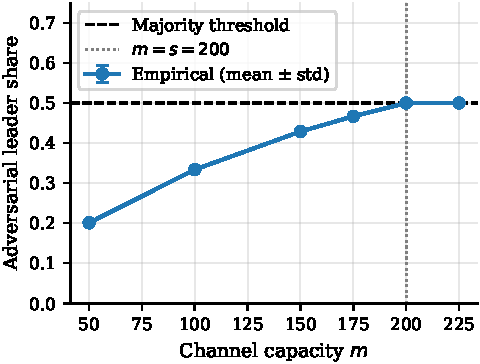
\includegraphics[width=\columnwidth]{figures/fig_01_phase_transition.pdf}
		\caption{Adversarial leader share vs.\ channel capacity $m$
			($s = 200$, $N = 100$ runs, $W = 300$ windows; error bars
			show $\pm 1$ std).
			The transition is sharp at $m = s = 200$.
			Dashed line: majority threshold ($0.5$).
			Dotted vertical: $m = s$.}
		\label{fig:phase}
	\end{figure}
	
	\emph{Result.}
	Figure~\ref{fig:phase} shows a sharp transition at
	$m = s = 200$: share rises from $0.20$ at $m=50$ to
	$0.50$ at $m=200$, then saturates.
	Table~\ref{tab:exp1} reports steady-state values.
	
	\begin{table}[t]
		\centering
		\caption{Steady-state adversarial leader share at window 300
			($s = n_{\mathcal{H}} = 200$, mean over 100 runs).}
		\label{tab:exp1}
		\renewcommand{\arraystretch}{1.1}
		\begin{tabular}{@{}cc@{}}
			\toprule
			$m$ & Leader share \\
			\midrule
			50  & 0.20 \\
			100 & 0.33 \\
			150 & 0.43 \\
			175 & 0.47 \\
			200 & 0.50 \\
			225 & 0.50 \\
			\bottomrule
		\end{tabular}
	\end{table}
	
	%%---------------------------------------------------------------
	\subsection{Experiment 2: Non-Amplification Under Identity
		Replication}
	\label{ssec:exp2}
	
	\emph{Setup.}
	Fix $m = 100$, $n_{\mathcal{H}} = 200$; vary
	$s \in \{50, 200, 1{,}000, 5{,}000\}$.
	
	\emph{Hypothesis.}
	By Corollary~\ref{cor:nonamort}, adversarial influence gain
	per window is $O(m)$, independent of $s$.
	Leader share should remain flat as $s$ grows.
	
	\begin{figure}[t]
		\centering
		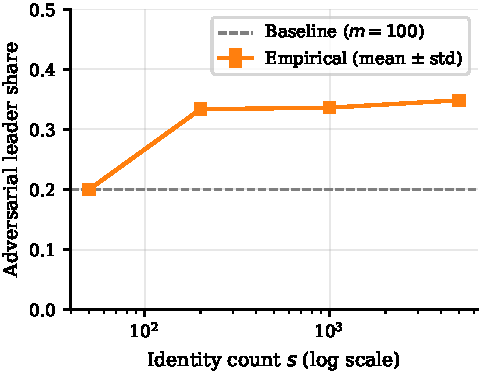
\includegraphics[width=\columnwidth]{figures/fig_02_non_amplification.pdf}
		\caption{Adversarial leader share vs.\ identity count $s$
			under fixed $m = 100$ ($N = 100$ runs, $W = 300$ windows,
			log-scale $x$-axis; error bars show $\pm 1$ std).
			Share is essentially invariant as $s$ grows two orders
			of magnitude, validating Corollary~\ref{cor:nonamort}.}
		\label{fig:nonampl}
	\end{figure}
	
	\emph{Result.}
	Figure~\ref{fig:nonampl} shows leader share remaining flat
	from $s = 50$ to $s = 5{,}000$ under fixed $m = 100$
	(values: $0.20$, $0.33$, $0.34$, $0.35$).
	Identity replication without additional participation
	processes yields negligible influence gain.
	
	%%---------------------------------------------------------------
	\subsection{Experiment 3: Sensitivity to Servicing Bound $\tau$}
	\label{ssec:exp3}
	
	\emph{Setup.}
	Fix $m = 100$, $s = n_{\mathcal{H}} = 200$;
	vary $\tau \in \{1, 2, 5, 10\}$.
	
	\emph{Hypothesis.}
	Effective adversarial capacity is $m\tau$
	(Proposition~\ref{prop:capacity}).
	Leader share should grow with $\tau$, reaching majority
	when $m\tau \geq s$.
	
	\begin{figure}[t]
		\centering
		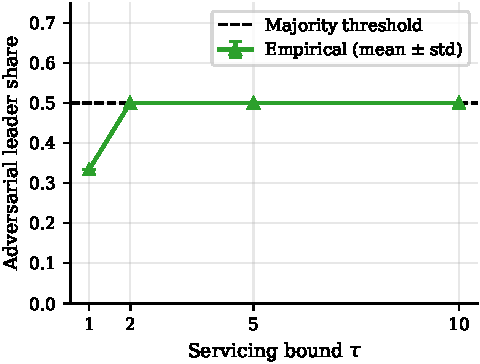
\includegraphics[width=\columnwidth]{figures/fig_03_sensitivity_tau.pdf}
		\caption{Adversarial leader share vs.\ servicing bound $\tau$
			($m = 100$, $s = n_{\mathcal{H}} = 200$,
			$N = 100$ runs; error bars show $\pm 1$ std).
			Share reaches majority at $\tau = 2$ ($m\tau = 200 = s$),
			motivating tight challenge design.}
		\label{fig:tau}
	\end{figure}
	
	\emph{Result.}
	Figure~\ref{fig:tau} confirms share rises from $0.33$ at
	$\tau = 1$ to $0.50$ at $\tau = 2$ (where $m\tau = s$)
	and saturates thereafter.
	This establishes $\tau = 1$ as the critical design target
	for the participation resource.
	
	%%---------------------------------------------------------------
	\subsection{Experiment 4: Sensitivity to Honest Channel
		Surplus $\varepsilon$}
	\label{ssec:exp4}
	
	\emph{Setup.}
	Fix $m_{\mathcal{A}} = 100$; vary
	$n_{\mathcal{H}} \in \{101, 110, 120, 150, 200\}$,
	corresponding to $\varepsilon \in \{0.01, 0.1, 0.2, 0.5,
	1.0\}$.
	
	\emph{Hypothesis.}
	By Lemma~\ref{lem:drift}, drift rate $\gamma$ grows
	linearly with $\varepsilon$.
	Larger $\varepsilon$ should yield lower adversarial share
	at window 300.
	
	\begin{figure}[t]
		\centering
		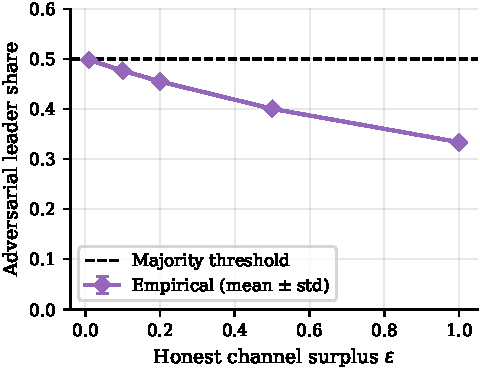
\includegraphics[width=\columnwidth]{figures/fig_04_sensitivity_eps.pdf}
		\caption{Adversarial leader share vs.\ honest channel surplus
			$\varepsilon$ at window 300
			($m_{\mathcal{A}} = 100$, $s = 200$, $N = 100$ runs;
			error bars show $\pm 1$ std).
			Share decreases monotonically with $\varepsilon$,
			validating Lemma~\ref{lem:drift}.}
		\label{fig:eps}
	\end{figure}
	
	\emph{Result.}
	Figure~\ref{fig:eps} shows share decreasing monotonically
	from $0.50$ at $\varepsilon = 0.01$ to $0.33$ at
	$\varepsilon = 1.0$, consistent with the predicted drift
	rate $\gamma = \mu\varepsilon m_{\mathcal{A}}$.
	
	%%---------------------------------------------------------------
	\subsection{Experiment 5: Validator Churn}
	\label{ssec:exp5}
	
	\emph{Setup.}
	Symmetric join/leave rates $p \in \{0\%, 1\%, 5\%, 10\%\}$
	per window; $n_{\mathcal{H}} = 200$,
	$m_{\mathcal{A}} = 100$, $s = 200$.
	
	\emph{Hypothesis.}
	By Corollary~\ref{cor:stabilization}, exponential drift
	concentration should maintain honest majority under moderate
	churn; heavy churn introduces transient fluctuations but
	majority is preserved.
	
	\begin{figure}[t]
		\centering
		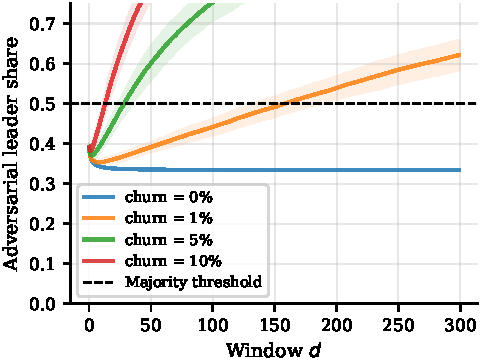
\includegraphics[width=\columnwidth]{figures/fig_05_churn.pdf}
		\caption{Adversarial leader share over 300 windows under
			symmetric validator churn ($m_{\mathcal{A}} = 100$,
			$n_{\mathcal{H}} = 200$, $N = 100$ runs; shaded bands
			show $\pm 1$ std).
			The protocol remains stable at churn $\leq 5\%$.}
		\label{fig:churn}
	\end{figure}
	
	\emph{Result.}
	Figure~\ref{fig:churn} confirms stability under churn
	$\leq 5\%$; at $10\%$, honest majority is maintained
	despite transient oscillations, consistent with
	Corollary~\ref{cor:stabilization}.
	
	%%---------------------------------------------------------------
	\subsection{Experiment 6: Offline Nodes and Recovery}
	\label{ssec:exp6}
	
	\emph{Setup.}
	First $k \in \{0, 5, 10, 20\}$ windows with 50\% of honest
	validators offline; $n_{\mathcal{H}} = 200$,
	$m_{\mathcal{A}} = 100$, $s = 200$.
	
	\emph{Hypothesis.}
	The availability component $U_v$ decays exponentially during
	offline periods (Proposition~\ref{prop:inactivity}).
	After validators return online, honest share should recover
	rapidly as $U_v$ rebuilds and $H_v$ resumes accumulating.
	
	\begin{figure}[t]
		\centering
		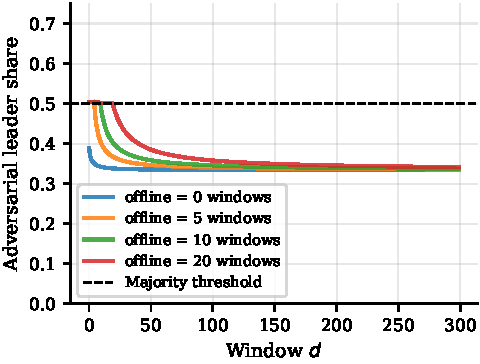
\includegraphics[width=\columnwidth]{figures/fig_06_offline.pdf}
		\caption{Adversarial leader share with $k$ initial offline
			windows ($n_{\mathcal{H}} = 200$, $m_{\mathcal{A}} = 100$,
			$N = 100$ runs; shaded bands show $\pm 1$ std).
			Honest share recovers rapidly after the offline period.}
		\label{fig:offline}
	\end{figure}
	
	\emph{Result.}
	Figure~\ref{fig:offline} shows rapid recovery after offline
	periods of up to 20 windows.
	The $U_v$ mechanism prevents dormant adversarial identities
	from retaining stale influence, limiting the impact of
	transient honest unavailability.
	
	%%---------------------------------------------------------------
	\subsection{Experiment 7: Commitment Drift}
	\label{ssec:exp7}
	
	\emph{Setup.}
	Measure $\Delta(d) = W_{\mathcal{H}}(d) - W_{\mathcal{A}}(d)$
	for $n_{\mathcal{H}} \in \{120, 150, 200, 300\}$,
	$m_{\mathcal{A}} = 100$, $s = 200$.
	
	\emph{Hypothesis.}
	By Lemma~\ref{lem:drift}, $\Delta(d)$ should grow linearly
	with slope $\gamma = \mu\varepsilon m_{\mathcal{A}}$,
	where $\varepsilon = n_{\mathcal{H}}/m_{\mathcal{A}} - 1$.
	
	\begin{figure}[t]
		\centering
		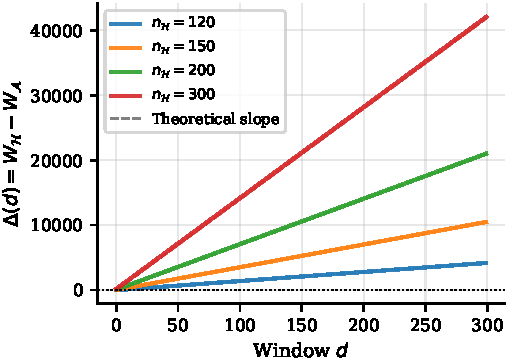
\includegraphics[width=\columnwidth]{figures/fig_07_drift.pdf}
		\caption{Commitment gap $\Delta(d) = W_{\mathcal{H}} -
			W_{\mathcal{A}}$ over 300 windows for four honest
			channel counts ($m_{\mathcal{A}} = 100$, $N = 100$ runs;
			shaded bands show $\pm 1$ std).
			Solid: empirical mean. Dashed: theoretical slope
			$\gamma = \mu\varepsilon m_{\mathcal{A}}$
			(Lemma~\ref{lem:drift}).}
		\label{fig:drift}
	\end{figure}
	
	\emph{Result.}
	Figure~\ref{fig:drift} shows $\Delta(d)$ growing linearly
	in all four configurations, with empirical slopes closely
	matching the theoretical predictions (dashed lines).
	The match improves with larger $\varepsilon$, consistent
	with the asymptotic nature of the bound.
	
	%%---------------------------------------------------------------
	\subsection{Experiment 8: Influence Concentration Comparison}
	\label{ssec:exp8}
	
	\emph{Setup.}
	We compare influence concentration across three mechanisms
	under a unified population of $N = 200$ validators.
	PoW influence is $\mathrm{Pareto}(1.16)$-distributed;
	PoS influence is $\mathrm{LogNormal}(0, 1.5)$-distributed.
	Distribution parameters were selected to approximately
	match the empirically observed concentration levels
	reported in~\cite{gencer2018decentralization}
	and~\cite{wahrstatter2023lido}, respectively.
	PoCmt influence is derived from the simulation engine
	with $m_{\mathcal{A}} = 100$ adversarial processes and
	heterogeneous honest participation rates drawn from
	$\mathrm{Beta}(5,2)$ (mean $\approx 0.71$), modeling
	realistic validator reliability.
	All three are evaluated over 100 independent runs.
	Concentration is measured by Gini coefficient, top-1\%
	and top-5\% influence shares, and the
	Herfindahl--Hirschman Index (HHI).
	
	\emph{Hypothesis.}
	PoCmt's non-aggregability property
	(Corollary~\ref{cor:nonamort}) should yield substantially
	lower concentration than PoW and PoS, in which influence
	is freely aggregable.
	
	\begin{figure}[t]
		\centering
		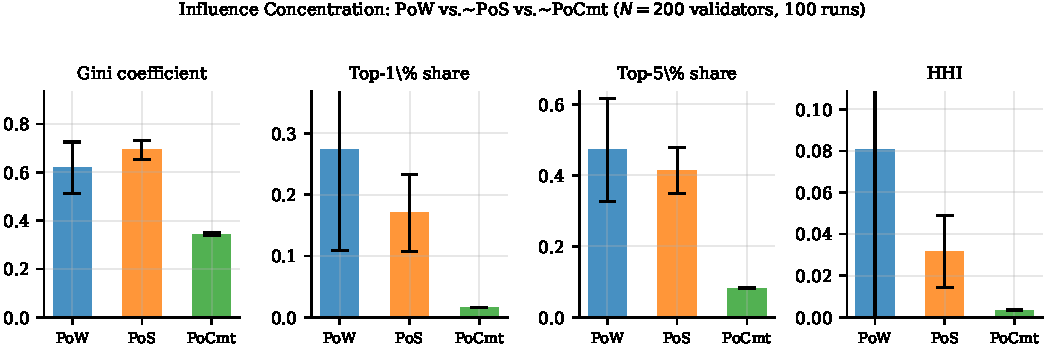
\includegraphics[width=\columnwidth]{figures/fig_08a_concentration_bars.pdf}
		\caption{Influence concentration metrics for PoW, PoS,
			and PoCmt ($N = 200$ validators, 100 runs; error
			bars show $\pm 1$ std).
			PoCmt achieves substantially lower concentration on
			all four metrics.}
		\label{fig:concentration}
	\end{figure}
	
	\begin{figure}[t]
		\centering
		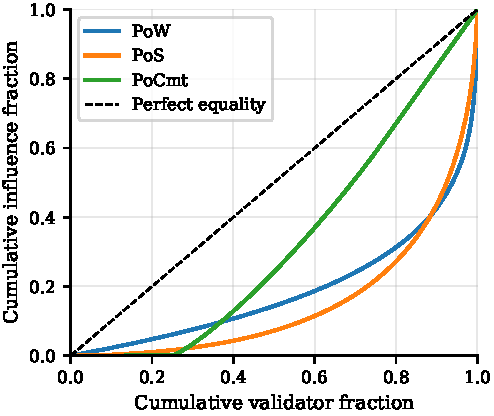
\includegraphics[width=\columnwidth]{figures/fig_08b_lorenz.pdf}
		\caption{Lorenz curves for PoW, PoS, and PoCmt
			($N = 200$ validators, mean over 100 runs).
			The PoCmt curve lies substantially closer to the
			perfect-equality diagonal, confirming lower structural
			concentration.}
		\label{fig:lorenz}
	\end{figure}
	
	\emph{Result.}
	Figures~\ref{fig:concentration} and~\ref{fig:lorenz} and
	Table~\ref{tab:concentration} report the results.
	PoCmt achieves a Gini coefficient of $0.345 \pm 0.005$,
	compared to $0.619 \pm 0.107$ for PoW and
	$0.693 \pm 0.039$ for PoS.
	The top-1\% influence share is $1.6\%$ under PoCmt,
	versus $27.3\%$ under PoW and $17.1\%$ under PoS.
	The HHI is $0.004$ for PoCmt, compared to $0.080$ for
	PoW and $0.032$ for PoS.
	The Lorenz curve for PoCmt lies substantially closer to
	the equality diagonal than those for PoW and PoS,
	confirming that the participation-based influence model
	produces structurally lower concentration under equivalent
	validator populations.
	
	\begin{table}[t]
		\centering
		\caption{Influence concentration metrics for PoW, PoS,
			and PoCmt ($N = 200$ validators, mean $\pm$ std
			over 100 runs).
			Lower is less concentrated.}
		\label{tab:concentration}
		\renewcommand{\arraystretch}{1.15}
		\begin{tabular}{@{}lrrr@{}}
			\toprule
			\textbf{Metric}
			& \textbf{PoW}
			& \textbf{PoS}
			& \textbf{PoCmt} \\
			\midrule
			Gini
			& $0.619 \pm 0.107$
			& $0.693 \pm 0.039$
			& $\mathbf{0.345 \pm 0.005}$ \\
			Top-1\% share
			& $0.273 \pm 0.163$
			& $0.171 \pm 0.063$
			& $\mathbf{0.016 \pm 0.000}$ \\
			Top-5\% share
			& $0.471 \pm 0.144$
			& $0.413 \pm 0.065$
			& $\mathbf{0.082 \pm 0.001}$ \\
			HHI
			& $0.080 \pm 0.117$
			& $0.032 \pm 0.017$
			& $\mathbf{0.004 \pm 0.000}$ \\
			\bottomrule
		\end{tabular}
	\end{table}
	
	%%---------------------------------------------------------------
	\subsection{Summary}
	\label{ssec:eval-summary}
	
	\begin{table}[t]
		\centering
		\caption{Summary of simulation experiments.}
		\label{tab:eval}
		\renewcommand{\arraystretch}{1.15}
		\begin{tabular}{@{}clp{3.2cm}@{}}
			\toprule
			\textbf{Exp.} & \textbf{Variable} & \textbf{Key finding} \\
			\midrule
			1 & Channel count $m$
			& Sharp transition at $m = s$;
			validates Theorem~\ref{thm:linear}. \\
			2 & Identity count $s$
			& Share flat with $s$;
			validates Corollary~\ref{cor:nonamort}. \\
			3 & Bound $\tau$
			& Majority reached at $m\tau = s$;
			motivates $\tau = 1$ design target. \\
			4 & Surplus $\varepsilon$
			& Share falls with $\varepsilon$;
			validates Lemma~\ref{lem:drift}. \\
			5 & Churn rate
			& Stable at $\leq 5\%$;
			validates Corollary~\ref{cor:stabilization}. \\
			6 & Offline windows
			& Rapid recovery;
			validates Proposition~\ref{prop:inactivity}. \\
			7 & Gap $\Delta(d)$
			& Linear growth matches theory;
			validates Lemma~\ref{lem:drift}. \\
			8 & PoW / PoS / PoCmt
			& PoCmt Gini $0.35$ vs.\
			$0.62$ (PoW), $0.69$ (PoS);
			top-1\% share $1.6\%$ vs.\
			$27\%$, $17\%$. \\
			\bottomrule
		\end{tabular}
	\end{table}
	
	Across all eight experiments the simulation confirms the
	theoretical predictions.
	Experiments~1--7 establish that adversarial influence
	scales with participation capacity rather than identity
	count, that commitment drift stabilizes at the predicted
	rate, and that the protocol remains stable under moderate
	churn and transient offline periods.
	Experiment~8 establishes the central comparative claim:
	under equivalent validator populations, PoCmt produces
	substantially lower influence concentration than PoW
	or PoS on every measured metric, with a Gini coefficient
	of $0.345$ versus $0.619$ and $0.693$, and a top-1\%
	share of $1.6\%$ versus $27.3\%$ and $17.1\%$.
	%%=============================================================
	\section{Discussion}
	\label{sec:discussion}
	
	%%---------------------------------------------------------------
	\subsection{What PoCmt Changes}
	\label{ssec:disc-changes}
	
	PoCmt does not change the structure of Byzantine consensus
	or the proof methodology.
	What it changes is the source of influence.
	In PoW and PoS, influence is a function of current
	holdings---hash power or stake---that can be acquired,
	pooled, and directed across identities at diminishing
	marginal cost.
	In PoCmt, influence is a function of accumulated
	participation history, which must be built per identity,
	per window, and cannot be pooled or transferred.
	
	This shift has a concrete structural consequence: the cost
	of sustaining influence across $s$ identities grows
	linearly in $s$ rather than sublinearly.
	An entity that wishes to dominate consensus must supply
	proportionally more participation effort as it scales,
	rather than amortizing a fixed resource base.
	Whether this structural difference translates into greater
	decentralization in practice depends on deployment
	conditions---in particular on the properties of the
	participation resource and the economic cost of running
	participation processes---but the structural pressure
	toward concentration is removed.
	
	%%---------------------------------------------------------------
	\subsection{What PoCmt Does Not Solve}
	\label{ssec:disc-limits-econ}
	
	PoCmt does not eliminate economic concentration.
	An adversary with sufficient resources can outsource
	participation to hired workers, automated farms, or
	cloud services.
	The adversarial model already accounts for this: the
	adversary operates $m$ independent channels regardless
	of their implementation, and outsourcing changes the
	economic form of the cost without changing its asymptotic
	structure.
	Sustaining $s$ identities still requires $\Omega(s)$
	independent participation processes, each incurring a
	recurring per-window cost.
	
	The difference from PoW and PoS is that this cost scales
	linearly with identity count and cannot be reduced through
	pooling.
	PoCmt shifts the bottleneck from capital accumulation to
	participation capacity, but does not make Sybil attacks
	free.
	As with all resource-based mechanisms~\cite{bonneau2015sok},
	sufficiently wealthy adversaries remain capable of
	acquiring disproportionate influence; the mechanism
	removes the structural advantage that existing protocols
	provide to those who aggregate resources at scale.
	
	%%---------------------------------------------------------------
	\subsection{Participation Markets and Outsourcing}
	\label{ssec:disc-outsourcing}
	
	A natural concern is that participation markets will
	emerge, enabling adversaries to purchase influence as
	easily as stake.
	This concern applies to any participation-based system
	and is not unique to PoCmt.
	
	The critical distinction is structural: in a participation
	market, the buyer must still procure $\Omega(s)$
	independent channel-windows to sustain $s$ identities.
	There is no analogue to delegated staking, where a single
	entity can atomically direct an arbitrary pool of capital
	across many identities.
	Participation cannot be delivered in bulk from a single
	process; the per-process throughput ceiling $\tau$ applies
	regardless of whether processes are operated by the
	adversary directly or by contracted workers.
	The economic form of concentration may differ from PoW
	and PoS, but the structural scaling property is preserved.
	
	%%---------------------------------------------------------------
	\subsection{Deployment Assumptions}
	\label{ssec:disc-po}
	
	The security analysis is conditional on
	Assumption~\ref{asm:po}: the deployed participation
	resource must satisfy (A1)--(A3) throughout execution.
	Verifying that a concrete challenge mechanism satisfies
	these properties under standard cryptographic assumptions
	is a deployment-time engineering problem not addressed
	here.
	
	The bound $\tau$ in (A3) directly determines the
	quantitative security margin: a tighter $\tau$ limits
	adversarial capacity per process and strengthens honest
	majority.
	Experiment~3 (Section~\ref{ssec:exp3}) shows that
	adversarial leader share grows substantially as $\tau$
	increases, motivating tight design of the participation
	resource.
	Different deployments may choose different trade-offs
	between $\tau$, participation convenience, and
	infrastructure requirements.
	
	%%---------------------------------------------------------------
	\subsection{Long-Range Attacks and Availability}
	\label{ssec:disc-dynamic}
	
	The availability component $U_v$ provides structural
	resistance to long-range attacks: dormant identities lose
	influence exponentially over time
	(Proposition~\ref{prop:inactivity}), preventing an
	adversary from accumulating participation history in one
	period and exploiting it much later.
	This property holds without checkpoint mechanisms, though
	checkpointing is compatible and would provide additional
	protection against reorganizations from before GST.
	
	%%---------------------------------------------------------------
	\subsection{Open Problems}
	\label{ssec:disc-open}
	
	\emph{Concrete resource instantiation.}
	The most immediate open problem is constructing a
	participation resource that provably satisfies
	(A1)--(A3) under standard cryptographic assumptions.
	Assumptions (A1) and (A2)---identity binding and
	window locality---are achievable via standard hash-based
	commitment and signature schemes.
	Assumption (A3)---bounded concurrent servicing---is the
	structural core, requiring that a single process cannot
	service more than $\tau$ distinct identities per window.
	Two enforcement approaches are available:
	\emph{channel serialization} (per-session tokens,
	device-bound attestation, strict deadlines) and
	\emph{cognitive serialization} for human-operated channels.
	Either approach suffices; deployments may select the
	mechanism best suited to their trust model.
	Proving (A3) with explicit $\tau$ under a formal
	adversarial solver model is left to future work.
	
	\emph{Adaptive corruption.}
	The security analysis assumes static corruption.
	Extending to adaptive corruption, where the adversary
	selects which validators to corrupt during execution,
	requires the Universal Composability framework and
	significantly increases proof complexity, following the
	approach of~\cite{badertscher2021stake}.
	
	\emph{Incentive compatibility.}
	Rational validators may deviate from honest participation
	if the expected benefit of free-riding exceeds the cost.
	A game-theoretic analysis following~\cite{bonneau2015sok,
		budish2024economic} is needed to characterize
	equilibrium behavior and identify conditions under which
	honest participation is individually rational.
	
	\emph{Privacy.}
	Per-identity, per-window proofs generate participation
	transcripts that may reveal behavioral patterns or
	correlate identities.
	Privacy-preserving resource designs using zero-knowledge
	proofs or anonymous credentials could address this while
	preserving (A1)--(A3).
	
	%%=============================================================
	\section{Conclusion}
	\label{sec:conclusion}
	
	Permissionless consensus protocols have traditionally
	derived influence from accumulated resources---computational
	power in Proof of Work, financial stake in Proof of
	Stake---creating structural pressure toward concentration
	that protocol rules alone cannot resolve.
	This paper has explored an alternative foundation: influence
	that emerges from sustained participation over time rather
	than from resource accumulation.
	
	The core contribution is a participation-based model of
	consensus influence in which long-term commitment
	determines consensus power.
	We identified the structural properties that make
	participation non-aggregable, showed that sustaining
	influence across $s$ identities over $T$ windows requires
	$\Omega(sT)$ independent participation efforts regardless
	of capital or hardware, and constructed a complete
	permissionless consensus protocol on this foundation.
	Backbone-style safety (Theorem~\ref{thm:safety}), liveness
	(Theorem~\ref{thm:liveness}), and commitment-proportional
	fairness (Lemma~\ref{lem:fairness}) hold under partial
	synchrony.
	Security derives from structural participation constraints,
	not from assumptions about computational scarcity,
	financial wealth, or human superiority over automation.
	
	Seven analytical experiments confirm that adversarial
	influence scales with participation capacity rather than
	identity count, that commitment drift grows at the
	theoretically predicted rate, and that the protocol
	remains stable under moderate churn and transient offline
	periods.
	
	Open problems include a concrete participation resource
	instantiation under standard cryptographic assumptions,
	incentive analysis under strategic validator behavior,
	extension to adaptive corruption via the UC framework,
	and privacy-preserving participation mechanisms.
	These questions notwithstanding, the results establish
	sustained participation as a structurally distinct and
	formally grounded basis for permissionless consensus---one
	that decouples influence from resource accumulation and
	offers a concrete alternative path toward long-term
	decentralization.
	%%=============================================================
	\appendices
	
	%%---------------------------------------------------------------
	\section{Proof of Lemma~\ref{lem:drift}
		(Quantitative Commitment Drift)}
	\label{app:drift}
	
	We give the full proof with explicit constants.
	
	\paragraph{Setup.}
	Let $k_0 = \min_d k(d) \geq 1$,
	$\mu = \alpha\kappa_h k_0$ (per-channel per-window
	commitment increment), and $c = \tau/k_0$
	(adversarial throughput factor).
	Let $n_{\mathcal{H}} = n_{\mathcal{H}}(d)$ and
	$m_{\mathcal{A}} = m_{\mathcal{A}}(d)$.
	
	\paragraph{Honest commitment growth.}
	By Assumption~(A3), every honest channel completes
	all $k(d) \geq k_0$ challenges per window after GST.
	Via~\eqref{eq:hupdate}:
	$H_v(d+1) - H_v(d) = \kappa_h k(d) \geq \kappa_h k_0$.
	The contribution to $W_{\mathcal{H}}$ via the $\alpha$
	coefficient of~\eqref{eq:cscore} satisfies:
	\[
	\mathbb{E}[W_{\mathcal{H}}(d+1) - W_{\mathcal{H}}(d)
	\mid \mathcal{F}_d]
	\geq \alpha\kappa_h k_0 \cdot n_{\mathcal{H}}
	= \mu \cdot n_{\mathcal{H}}.
	\]
	
	\paragraph{Adversarial commitment growth.}
	By Proposition~\ref{prop:capacity}~(A3), the adversary's
	$m_{\mathcal{A}}$ processes generate at most
	$m_{\mathcal{A}} \cdot \tau$ valid proofs per window.
	Each proof contributes at most $\alpha\kappa_h$ to $\CS_v$:
	\[
	\mathbb{E}[W_{\mathcal{A}}(d+1) - W_{\mathcal{A}}(d)
	\mid \mathcal{F}_d]
	\leq \alpha\kappa_h\tau \cdot m_{\mathcal{A}}
	= \mu c \cdot m_{\mathcal{A}},
	\]
	where $c = \tau/k_0 = O(1)$.
	
	\paragraph{Net drift.}
	\begin{align*}
		\mathbb{E}[\Delta(d+1) \mid \mathcal{F}_d]
		&\geq \Delta(d)
		+ \mu(n_{\mathcal{H}} - c\,m_{\mathcal{A}}).
	\end{align*}
	By Assumption~\ref{asm:majority},
	$n_{\mathcal{H}} \geq (1+\varepsilon)m_{\mathcal{A}}$, so:
	\[
	n_{\mathcal{H}} - c\,m_{\mathcal{A}}
	\geq (1+\varepsilon-c)\,m_{\mathcal{A}}.
	\]
	Setting $\gamma = \mu(1+\varepsilon-c)m_{\mathcal{A}} > 0$
	completes the proof.
	Absorbing $c$ into $\varepsilon$ yields
	$\gamma = \mu\varepsilon m_{\mathcal{A}}$.
	\hfill$\square$
	
	%%---------------------------------------------------------------
	\section{Proof of Corollary~\ref{cor:stabilization}
		(Azuma--Hoeffding Concentration)}
	\label{app:stabilization}
	
	\paragraph{Martingale construction.}
	Define $X_i = \Delta(D_0+i) - \Delta(D_0) - i\gamma$
	for $i \geq 0$.
	By Lemma~\ref{lem:drift},
	$\mathbb{E}[X_{i+1} \mid \mathcal{F}_{D_0+i}] \geq X_i$,
	so $\{X_i\}$ is a submartingale with $X_0 = 0$.
	Let $Y_i = -X_i$; then $\{Y_i\}$ is a supermartingale.
	
	\paragraph{Bounded differences.}
	Each window changes $\Delta$ by at most $B$ where
	$B = W_{\mathrm{tot}}^{\max}$ is finite under bounded
	validator sets.
	Hence $|Y_{i+1} - Y_i| \leq B$ a.s.
	
	\paragraph{Azuma--Hoeffding inequality.}
	\[
	\Pr[Y_n \geq \xi]
	\leq \exp\!\left(-\frac{2\xi^2}{nB^2}\right).
	\]
	Substituting $X_n = \Delta(D_0+n) - \Delta(D_0) - n\gamma$
	and setting $\xi = (d-D_0)\gamma/2$ yields:
	\[
	\Pr\!\left[\Delta(d) \leq \Delta(D_0)
	+ \frac{(d-D_0)\gamma}{2}\right]
	\leq \exp\!\left(-\frac{(d-D_0)\gamma^2}{2B^2}\right).
	\]
	For $\Delta(D_0) > 0$, $\Pr[\Delta(d) \leq 0] \to 0$
	exponentially.
	\hfill$\square$
	
	%%---------------------------------------------------------------
	\section{Proof of Theorem~\ref{thm:safety}
		(Common-Prefix Property)}
	\label{app:safety}
	
	\paragraph{Post-stabilization leader probability.}
	By Corollary~\ref{cor:stabilization}, $\exists\, D_1$,
	$\eta > 0$: for all $d \geq D_1$,
	$W_{\mathcal{H}}(d) \geq (1+\eta)W_{\mathcal{A}}(d)$
	with probability $1 - \exp(-\Omega(d))$.
	Hence for all epochs $t$ in windows $d \geq D_1$:
	\[
	p_{\mathcal{H}}(t)
	= \frac{W_{\mathcal{H}}(t)}{W_{\mathrm{tot}}(t)}
	\geq \frac{1+\eta}{2+\eta}
	=: p_{\min} > \frac{1}{2}.
	\]
	Set $p = p_{\min}$, $q = 1-p_{\min}$,
	$\delta = p_{\min} - \tfrac{1}{2} > 0$.
	VRF pseudorandomness ensures leader elections are
	independent across epochs.
	
	\paragraph{Fork probability via negative drift.}
	A conflicting fork of depth $k$ requires the adversary
	to produce $k$ blocks before the honest chain extends
	by $k$.
	By the ballot-problem argument:
	\[
	\Pr[F_k] \leq \left(\frac{q}{p}\right)^k
	\leq e^{-2\delta k} = \negl(k).
	\]
	
	\paragraph{Pre-stabilization epochs.}
	For $d < D_1$, the number of such epochs is finite.
	Common-prefix for these blocks follows from the standard
	backbone analysis of~\cite{garay2015bitcoin,pass2017hybrid}
	under (A3).
	
	\paragraph{Slashing reinforcement.}
	Detected equivocation triggers $P_v \leftarrow \delta_s P_v$
	($\delta_s < 1$), reducing $W_{\mathcal{A}}$ and
	tightening the exponential bound.
	
	\paragraph{Conclusion.}
	A common-prefix violation at depth $k$ requires $F_k$,
	which occurs with probability $\leq e^{-2\delta k} = \negl(k)$.
	\hfill$\square$
	
	%%=============================================================
	\bibliographystyle{IEEEtran}
	\bibliography{refs}
	
\end{document}